\section{Construction}
The team was given several weeks to spend on constructing the motor-generator set.

    \subsection{Brainstorming Phase}
    Construction for the motor-generator project began with a very simple prototype to demonstrate an understanding of electromagnetic induction. A simple copper coil was balanced on conductive paper clips connected to a battery supplying direct current via breadboards. Ceramic magnets were placed under the coil. When the circuit was completed, the coil would rotate due to the induced magnetic fields in it. When the power source was replaced with a voltmeter, the coil was manually rotated to induce up to 40 mV.

    \begin{figure}[ht]
        \begin{center}
            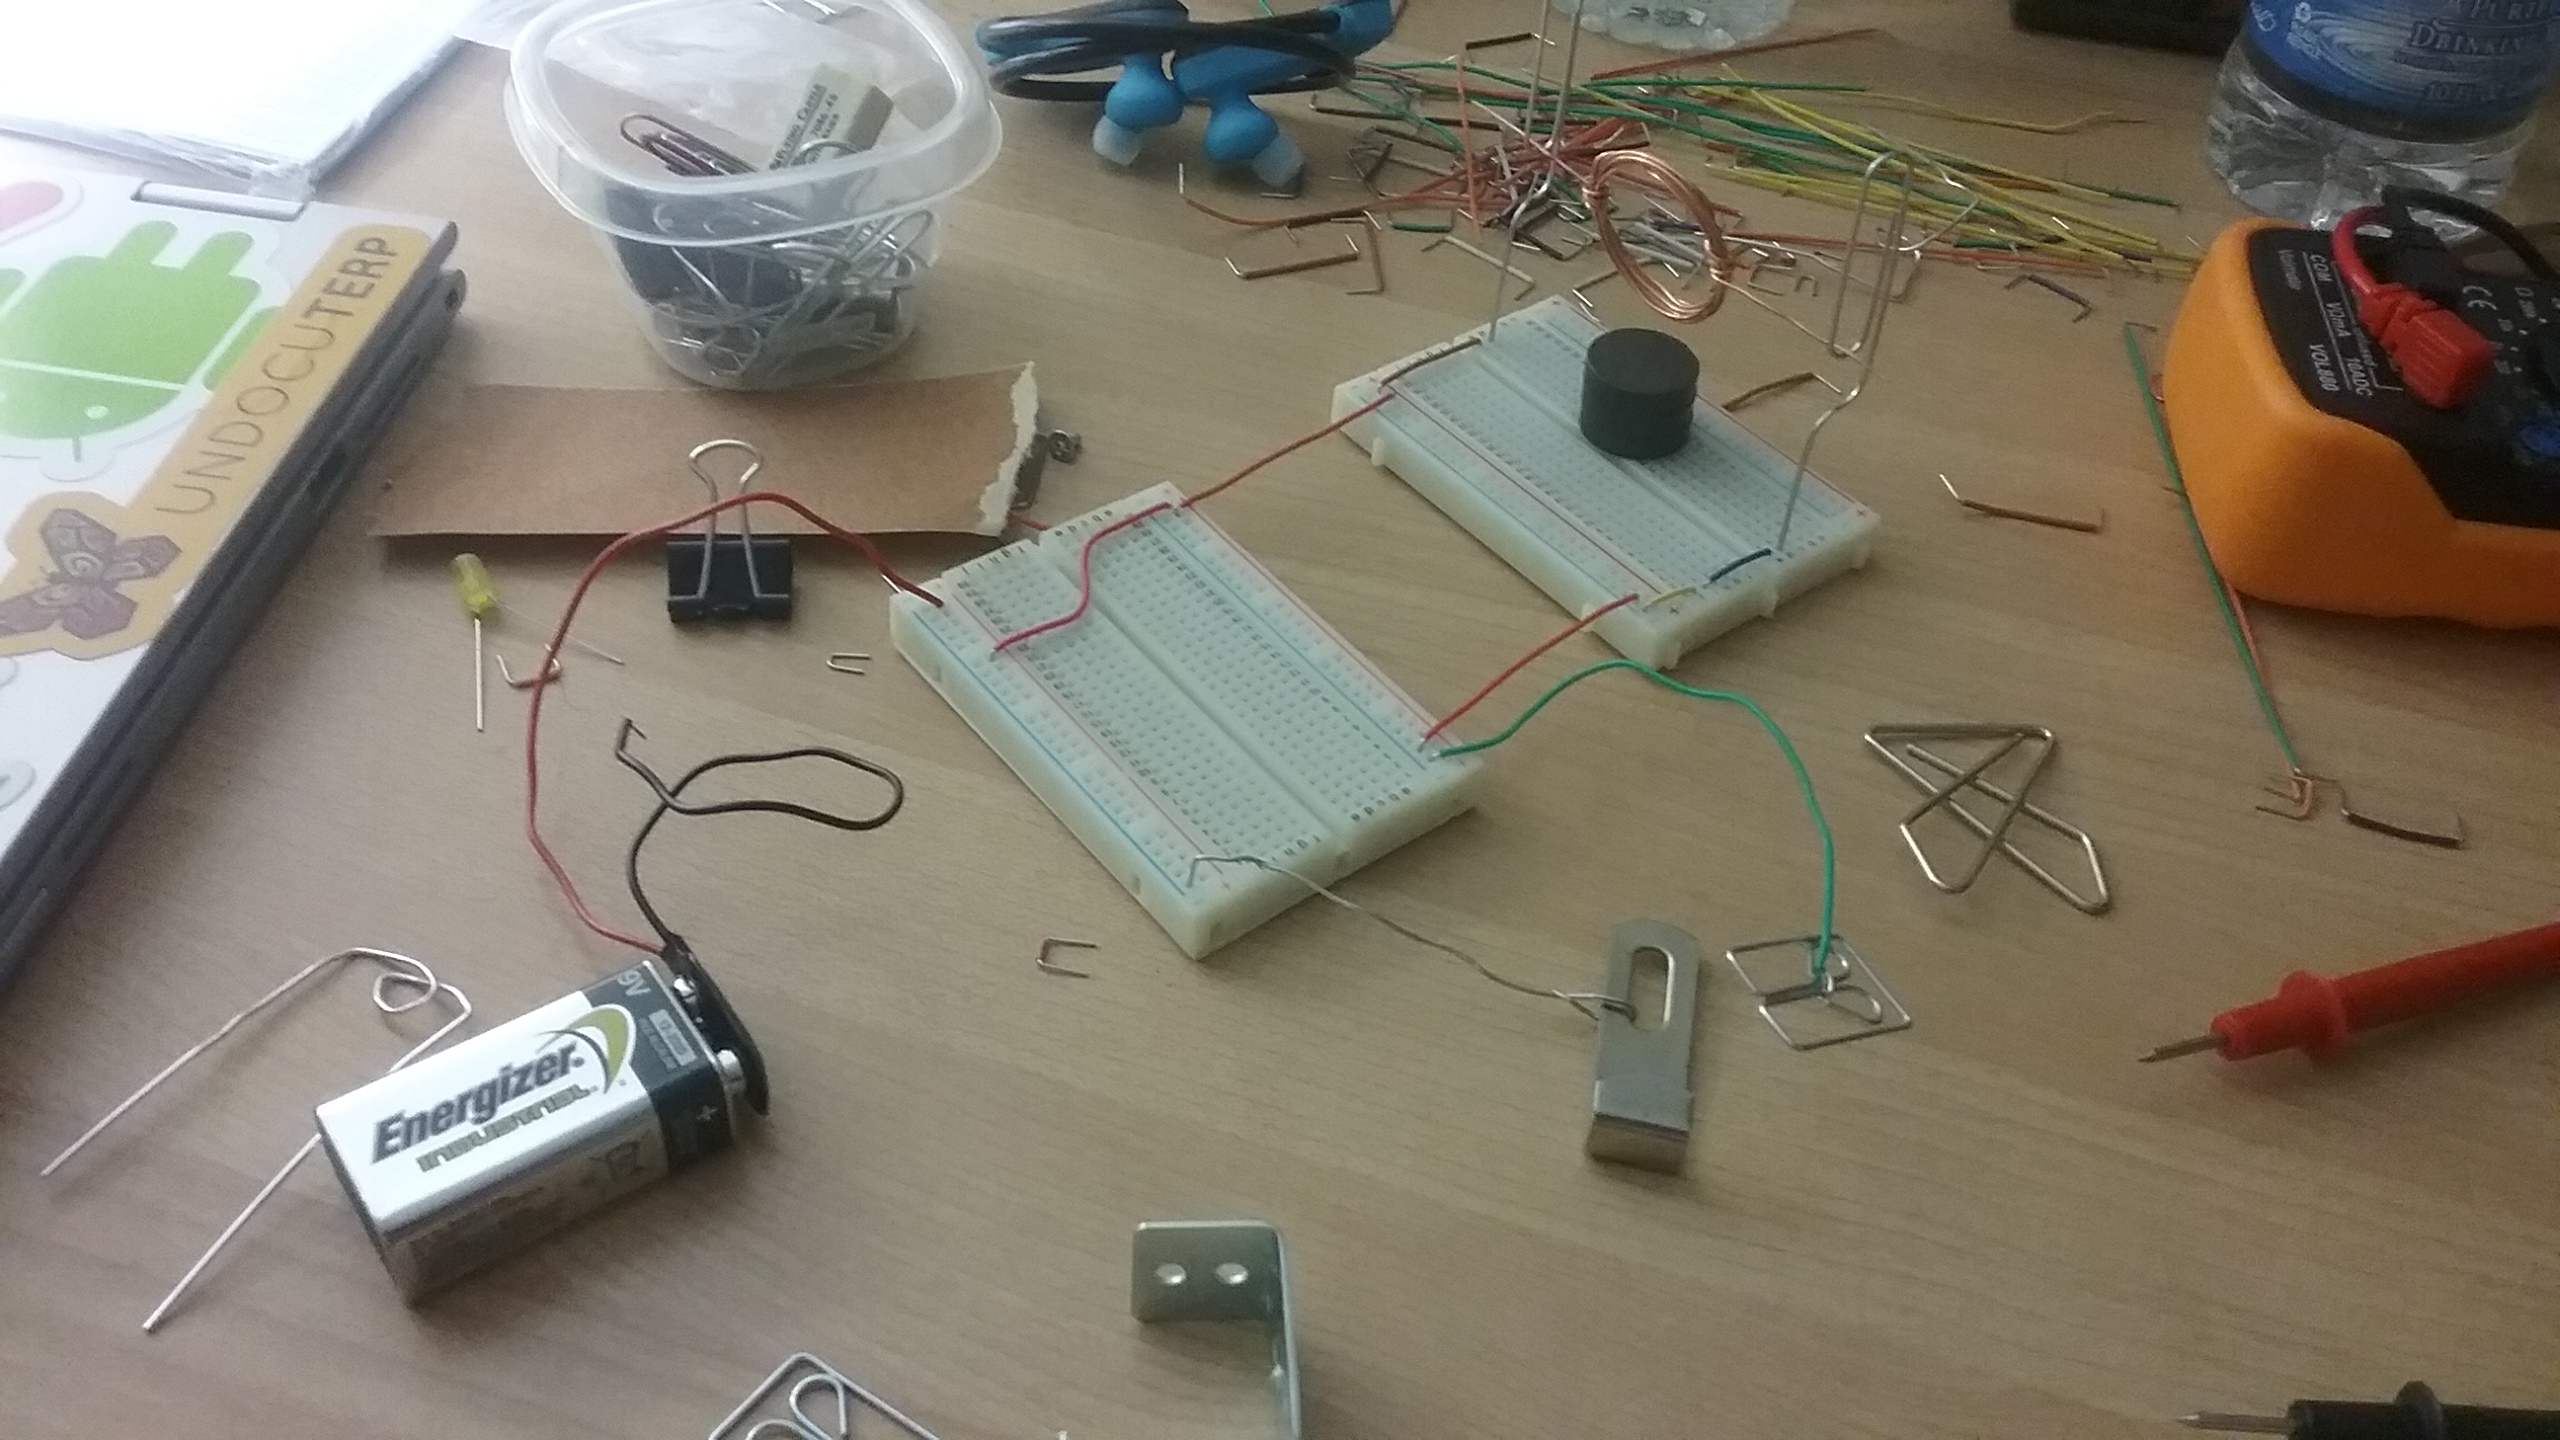
\includegraphics[width=0.5\textwidth]{figures/models/1.jpg}
            \label{fig:model1}
        \end{center} \caption{Simple Prototype}
    \end{figure}

    \subsection{Multiple Trials}
    Creating a model with a spinning coil appeared feasible, until the team realized its lack of mechanical engineering skills and its lack of experience with machine tools beyond a power drill. The coil was upgraded, along with the strength of the magnets and the input power. However, due to an unbalanced coil, poor choices of materials and a flimsy frame, the model failed to yield any results.\\

    \begin{figure}[ht]
        \begin{center}
            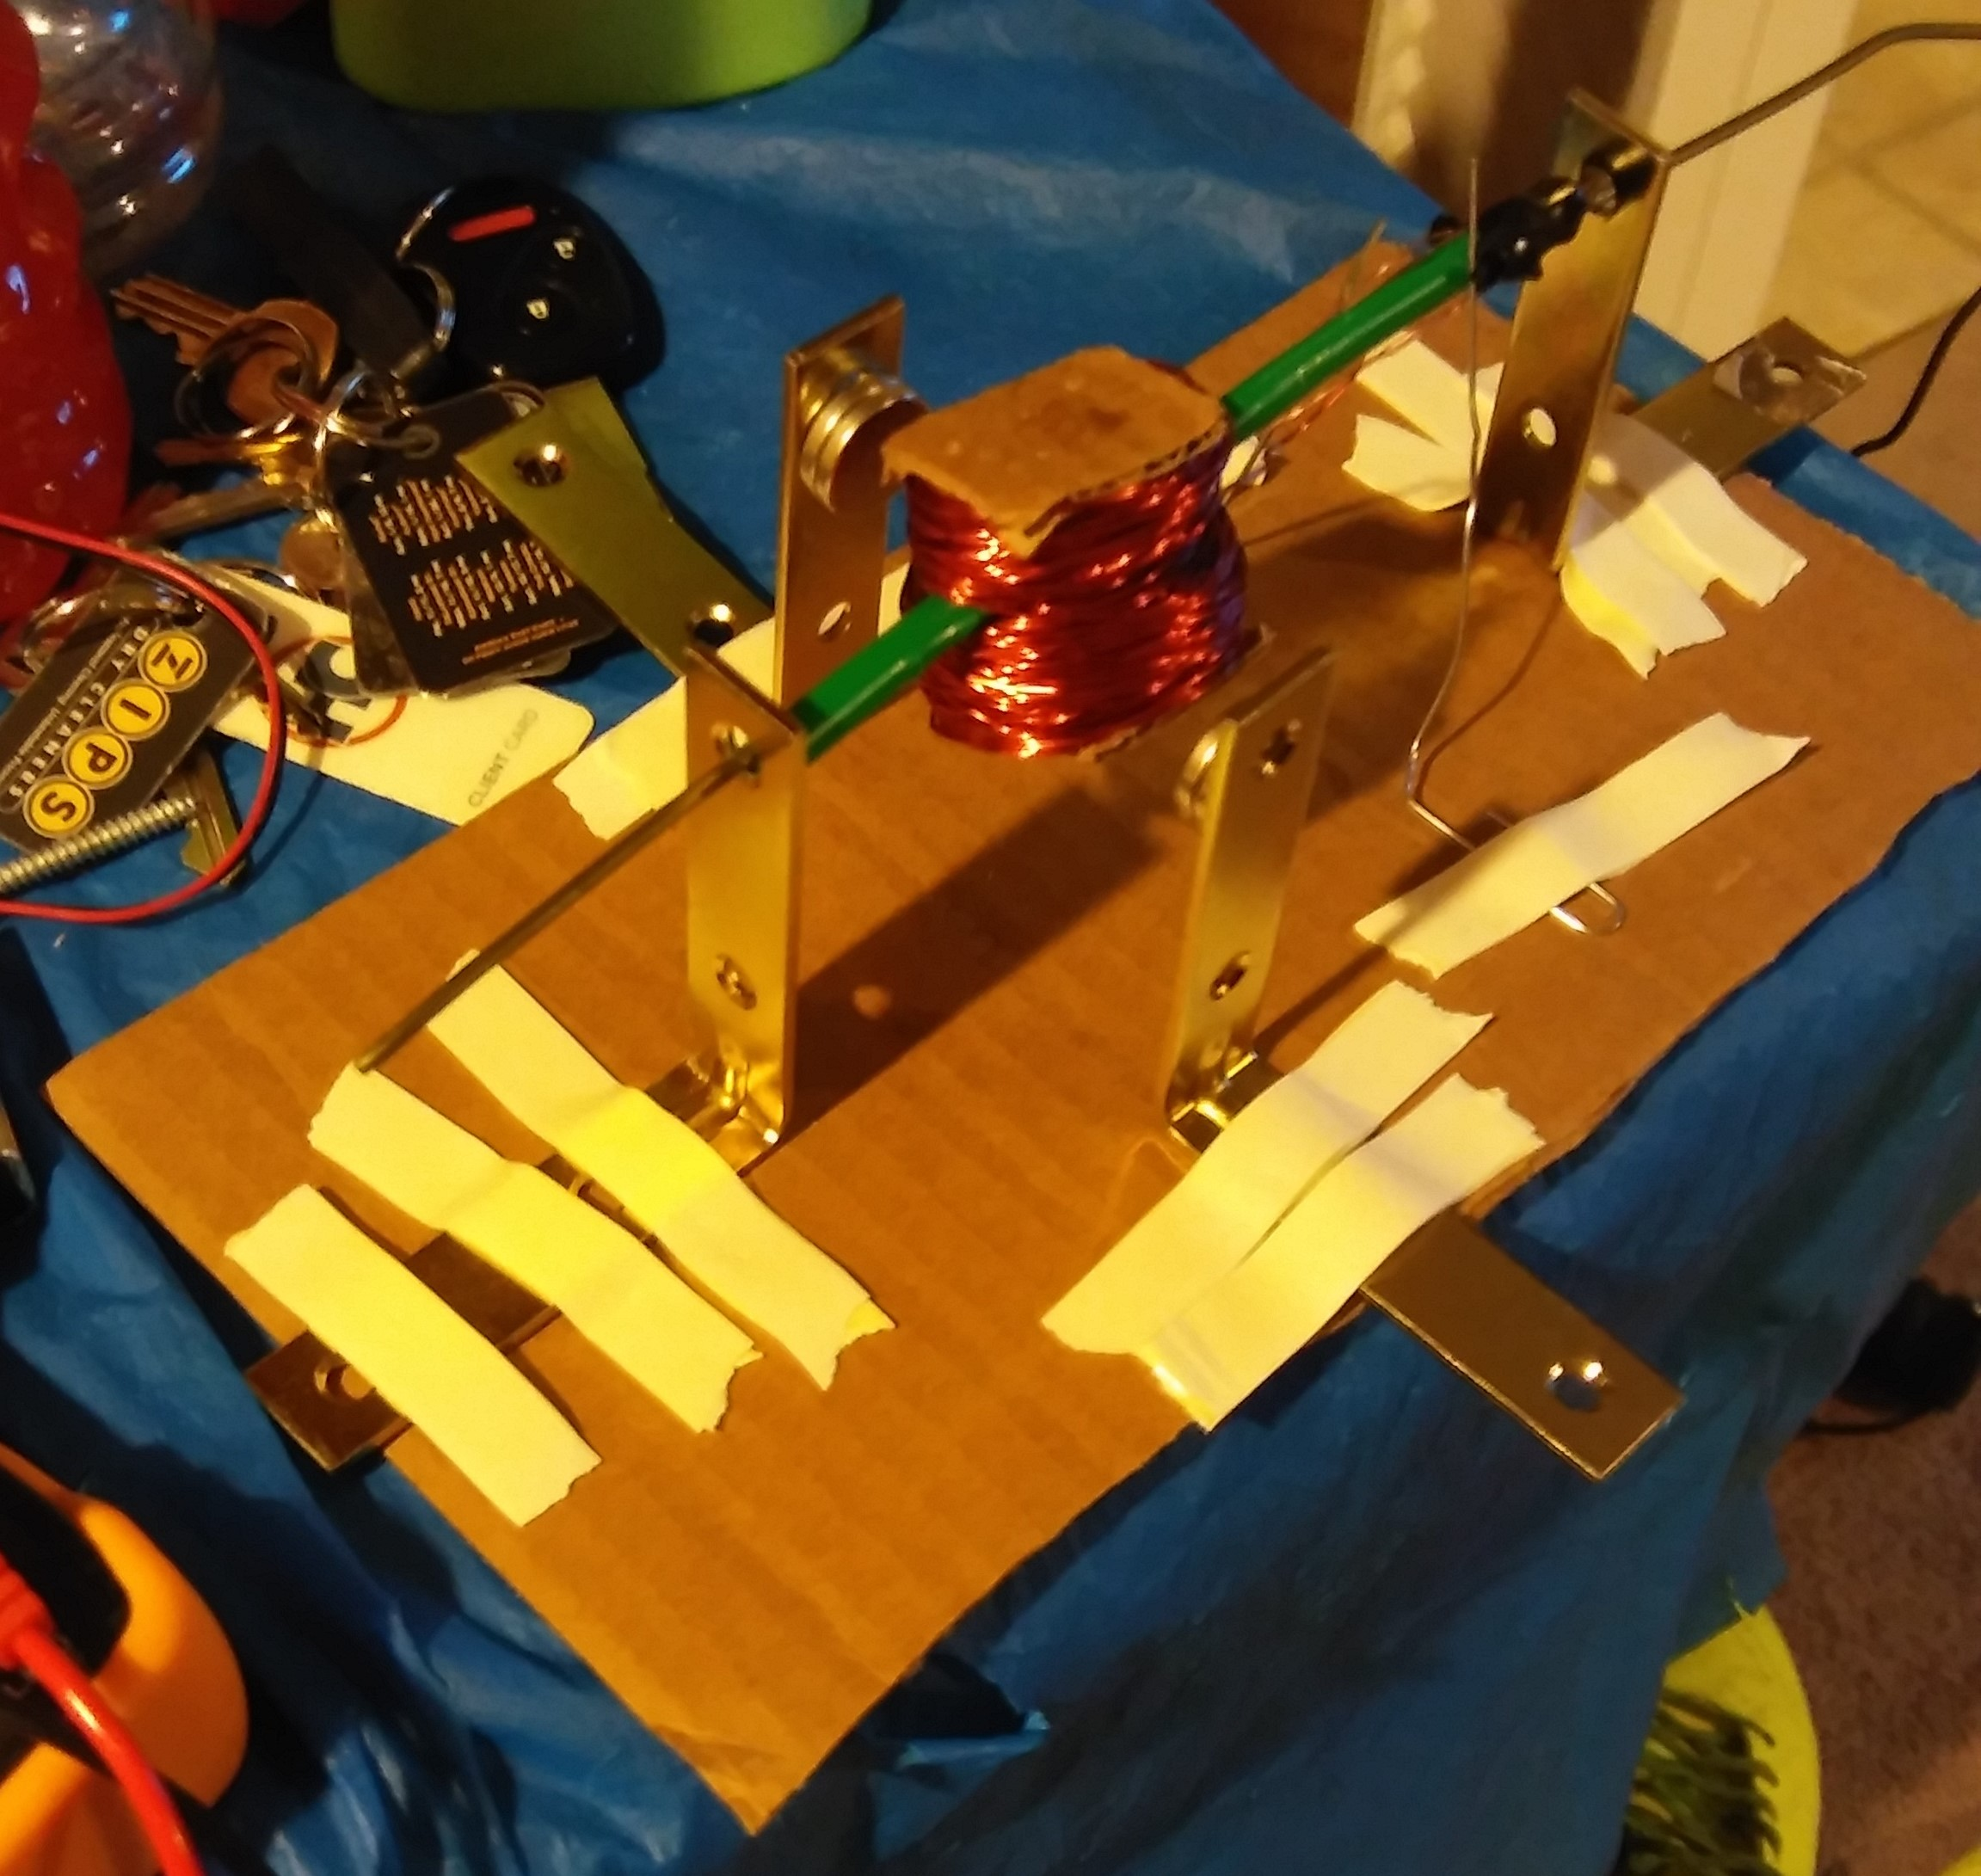
\includegraphics[width=0.5\textwidth]{figures/models/2.jpg}
            \label{fig:model2}
        \end{center} \caption{Upgraded Coil Model}
    \end{figure}

    \noindent
    Since balancing the coil proved to be a challenging task by itself, the neodymium magnets became the rotating apparatus in the next design. Magnetic wire was used to coil around an iron hook, with the magnets attached to the armature. Theoretically, the magnetic fields rotating perpendicularly through the coils would generate current. The design however failed to generate sufficient current through the narrow strip of coils.\\

    \begin{figure}[ht]
        \begin{center}
            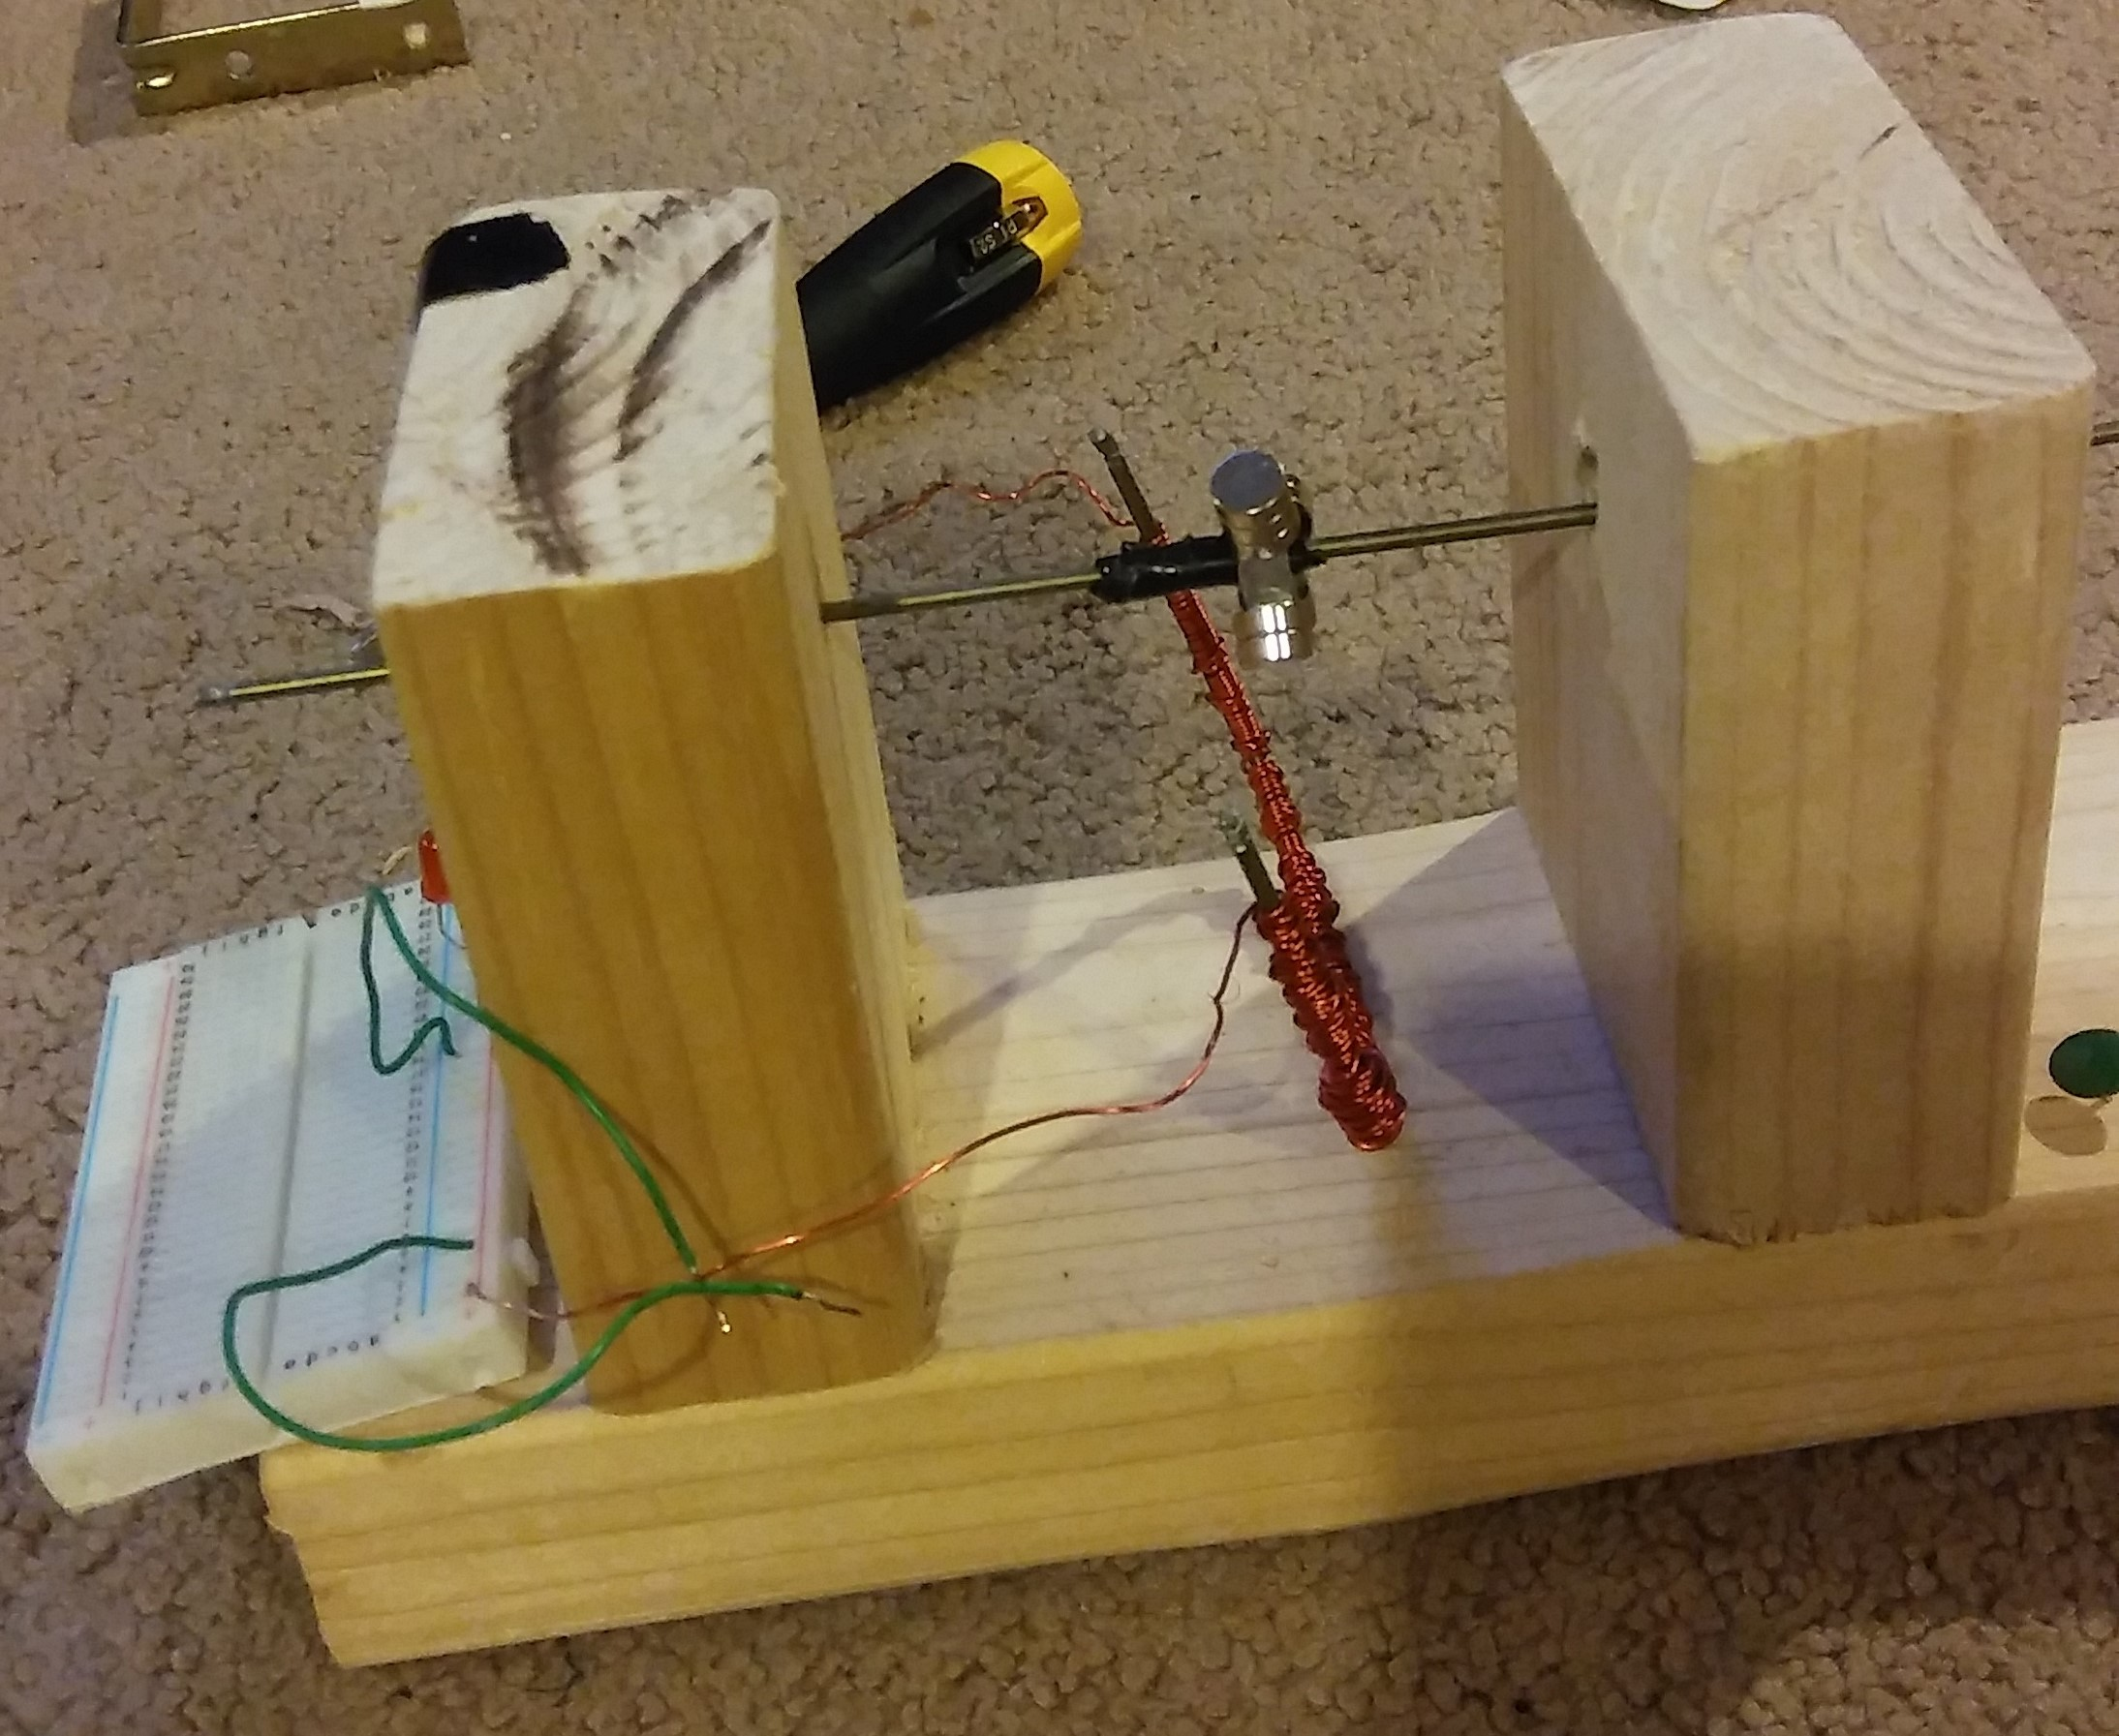
\includegraphics[width=0.5\textwidth]{figures/models/3.jpg}
            \label{fig:model3}
        \end{center} \caption{Spinning Magnetic Fields}
    \end{figure}

    \noindent
    A different orientation of the coils were tested and quickly discarded.

    \begin{figure}[ht]
        \begin{center}
            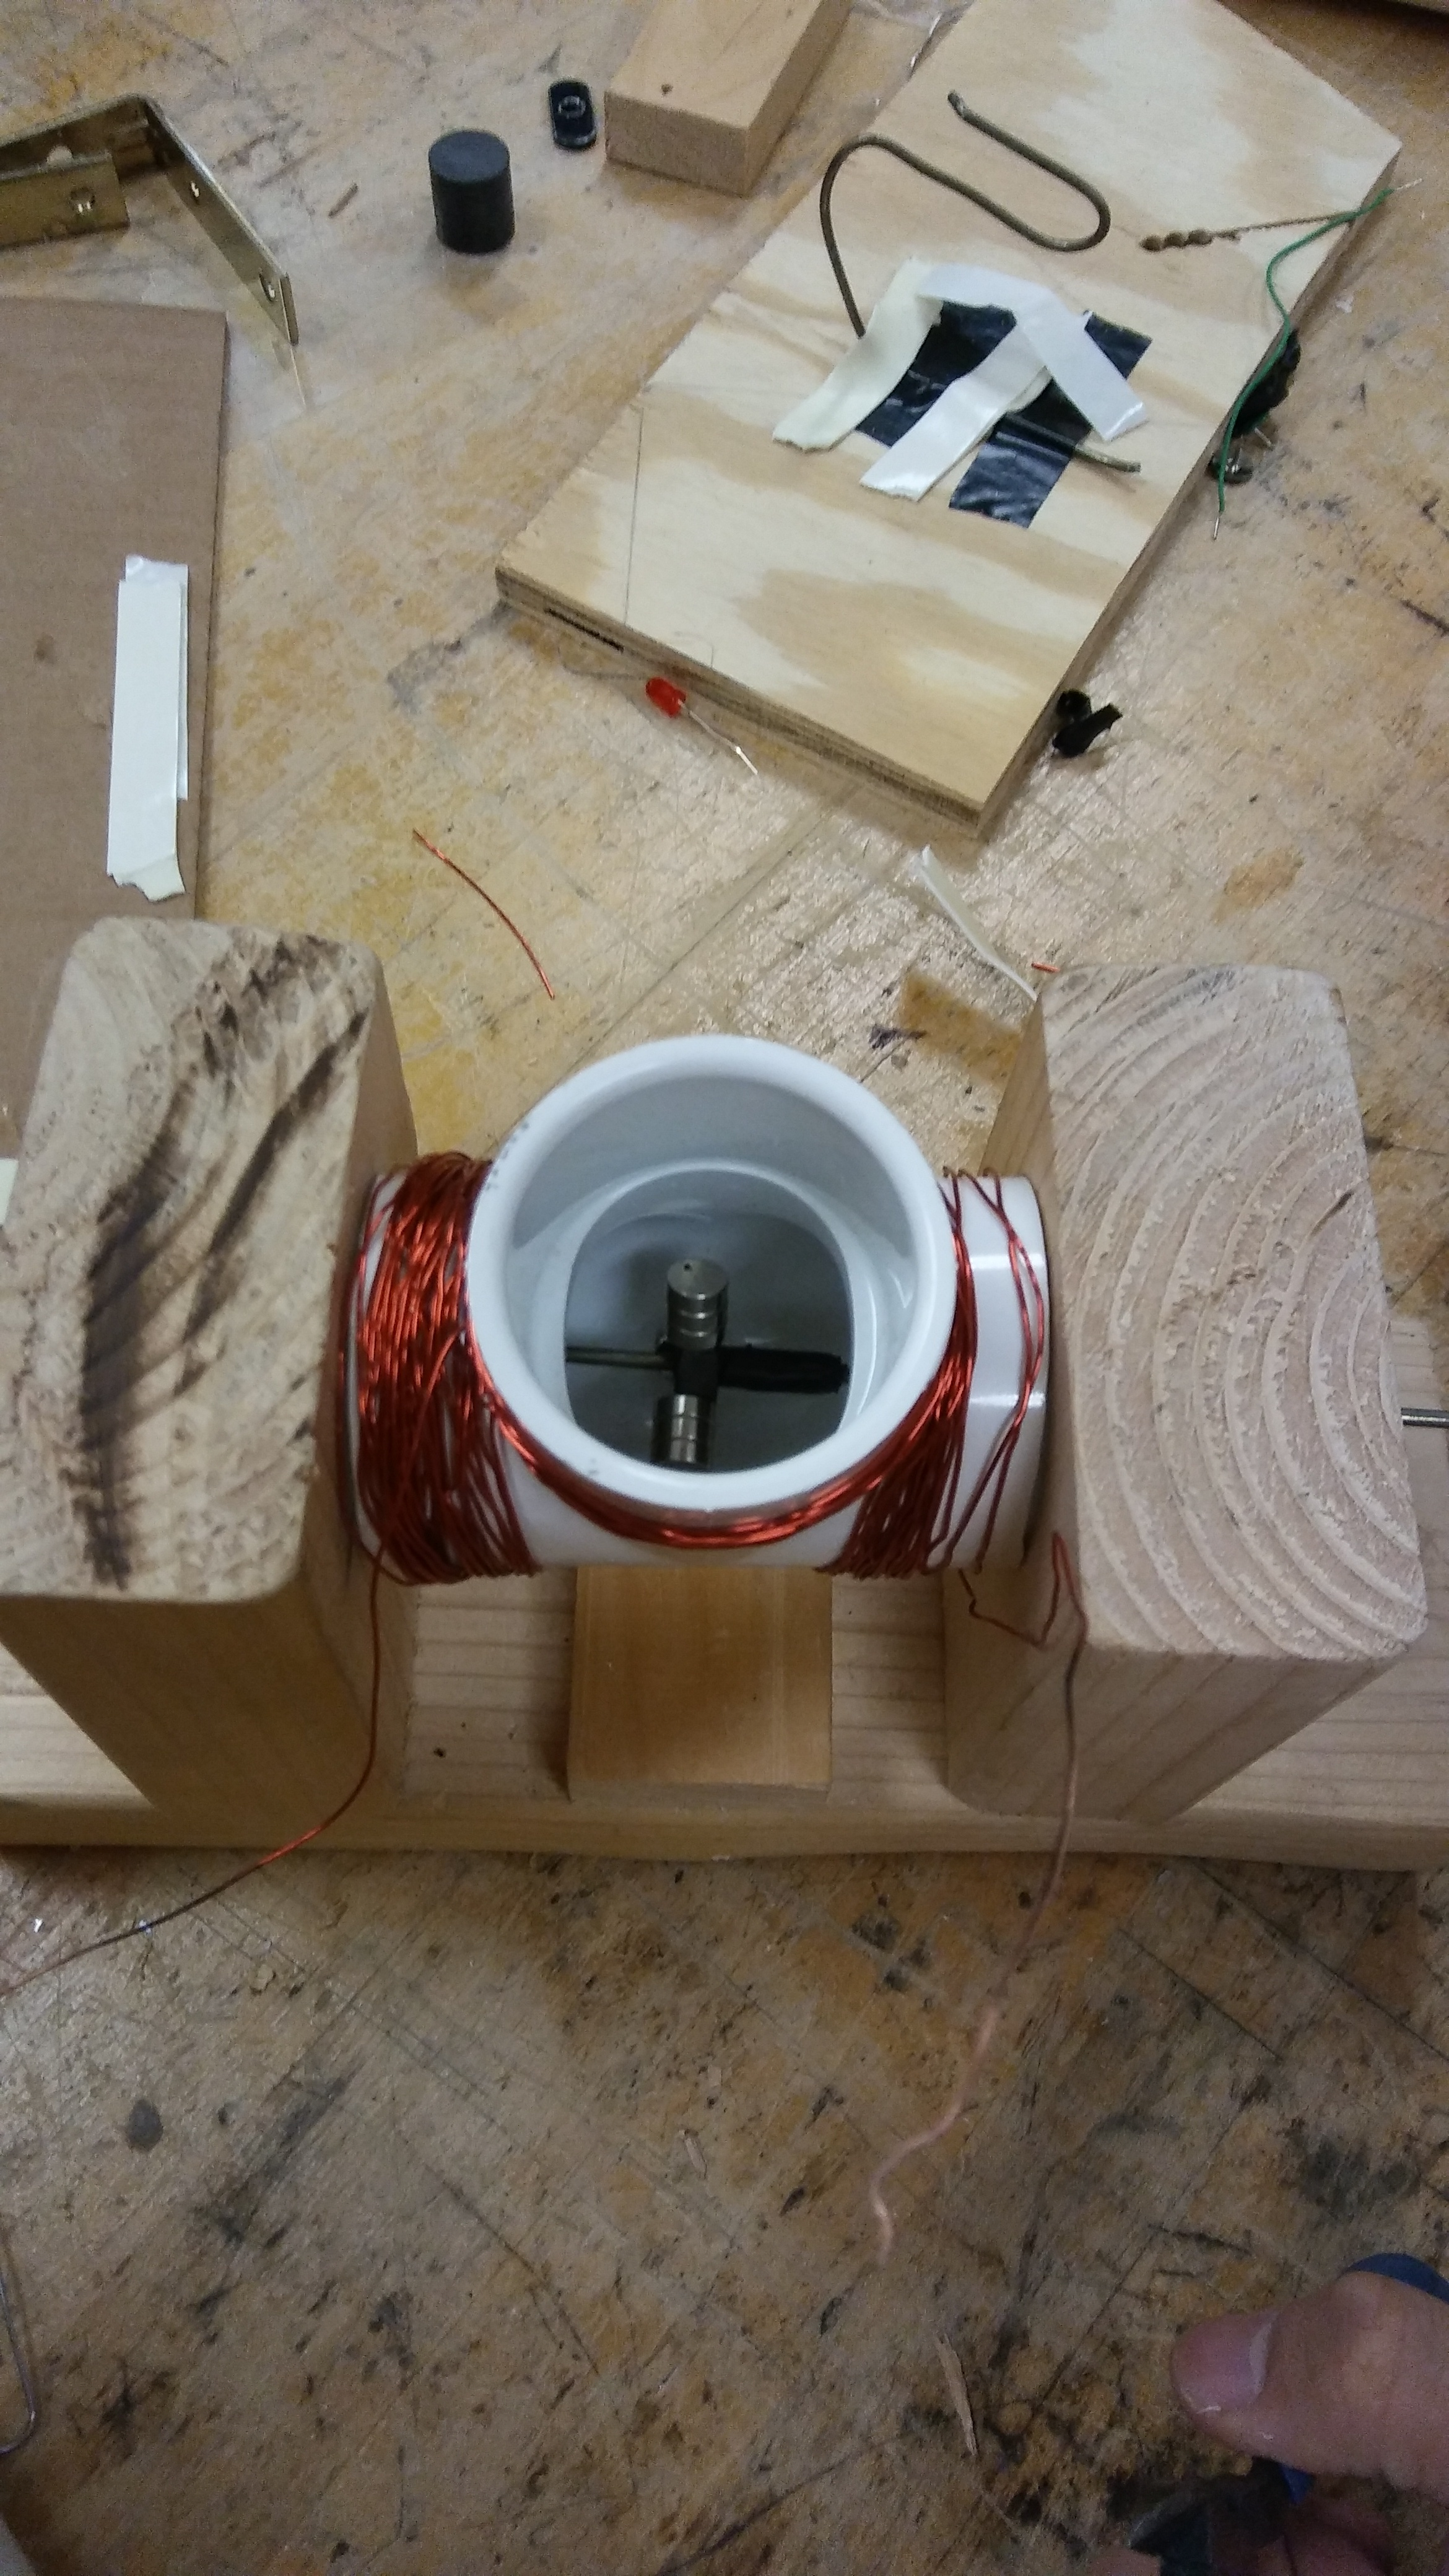
\includegraphics[width=0.5\textwidth]{figures/models/4.jpg}
            \label{fig:model4}
        \end{center} \caption{Spinning Magnetic Fields with Coils in Multiple Orientations}
    \end{figure}

    \subsection{Final Model}
    The narrow strip of coils was upgraded to provide more surface area for the magnetic fields to interact with. The design however did not yield results consistently. Supplying power would only cause the armature to twitch, which may be due to the wire not being tightly coiled, the wire not having ideal conductive properties as expected, or the 9 V input being insufficient. When spinning the armature, a voltmeter would occasionally read minor outputs. Nevertheless, the model failed to achieve the expected results when demonstrated during the team's presentation.\\

    \begin{figure}[ht]
        \begin{center}
            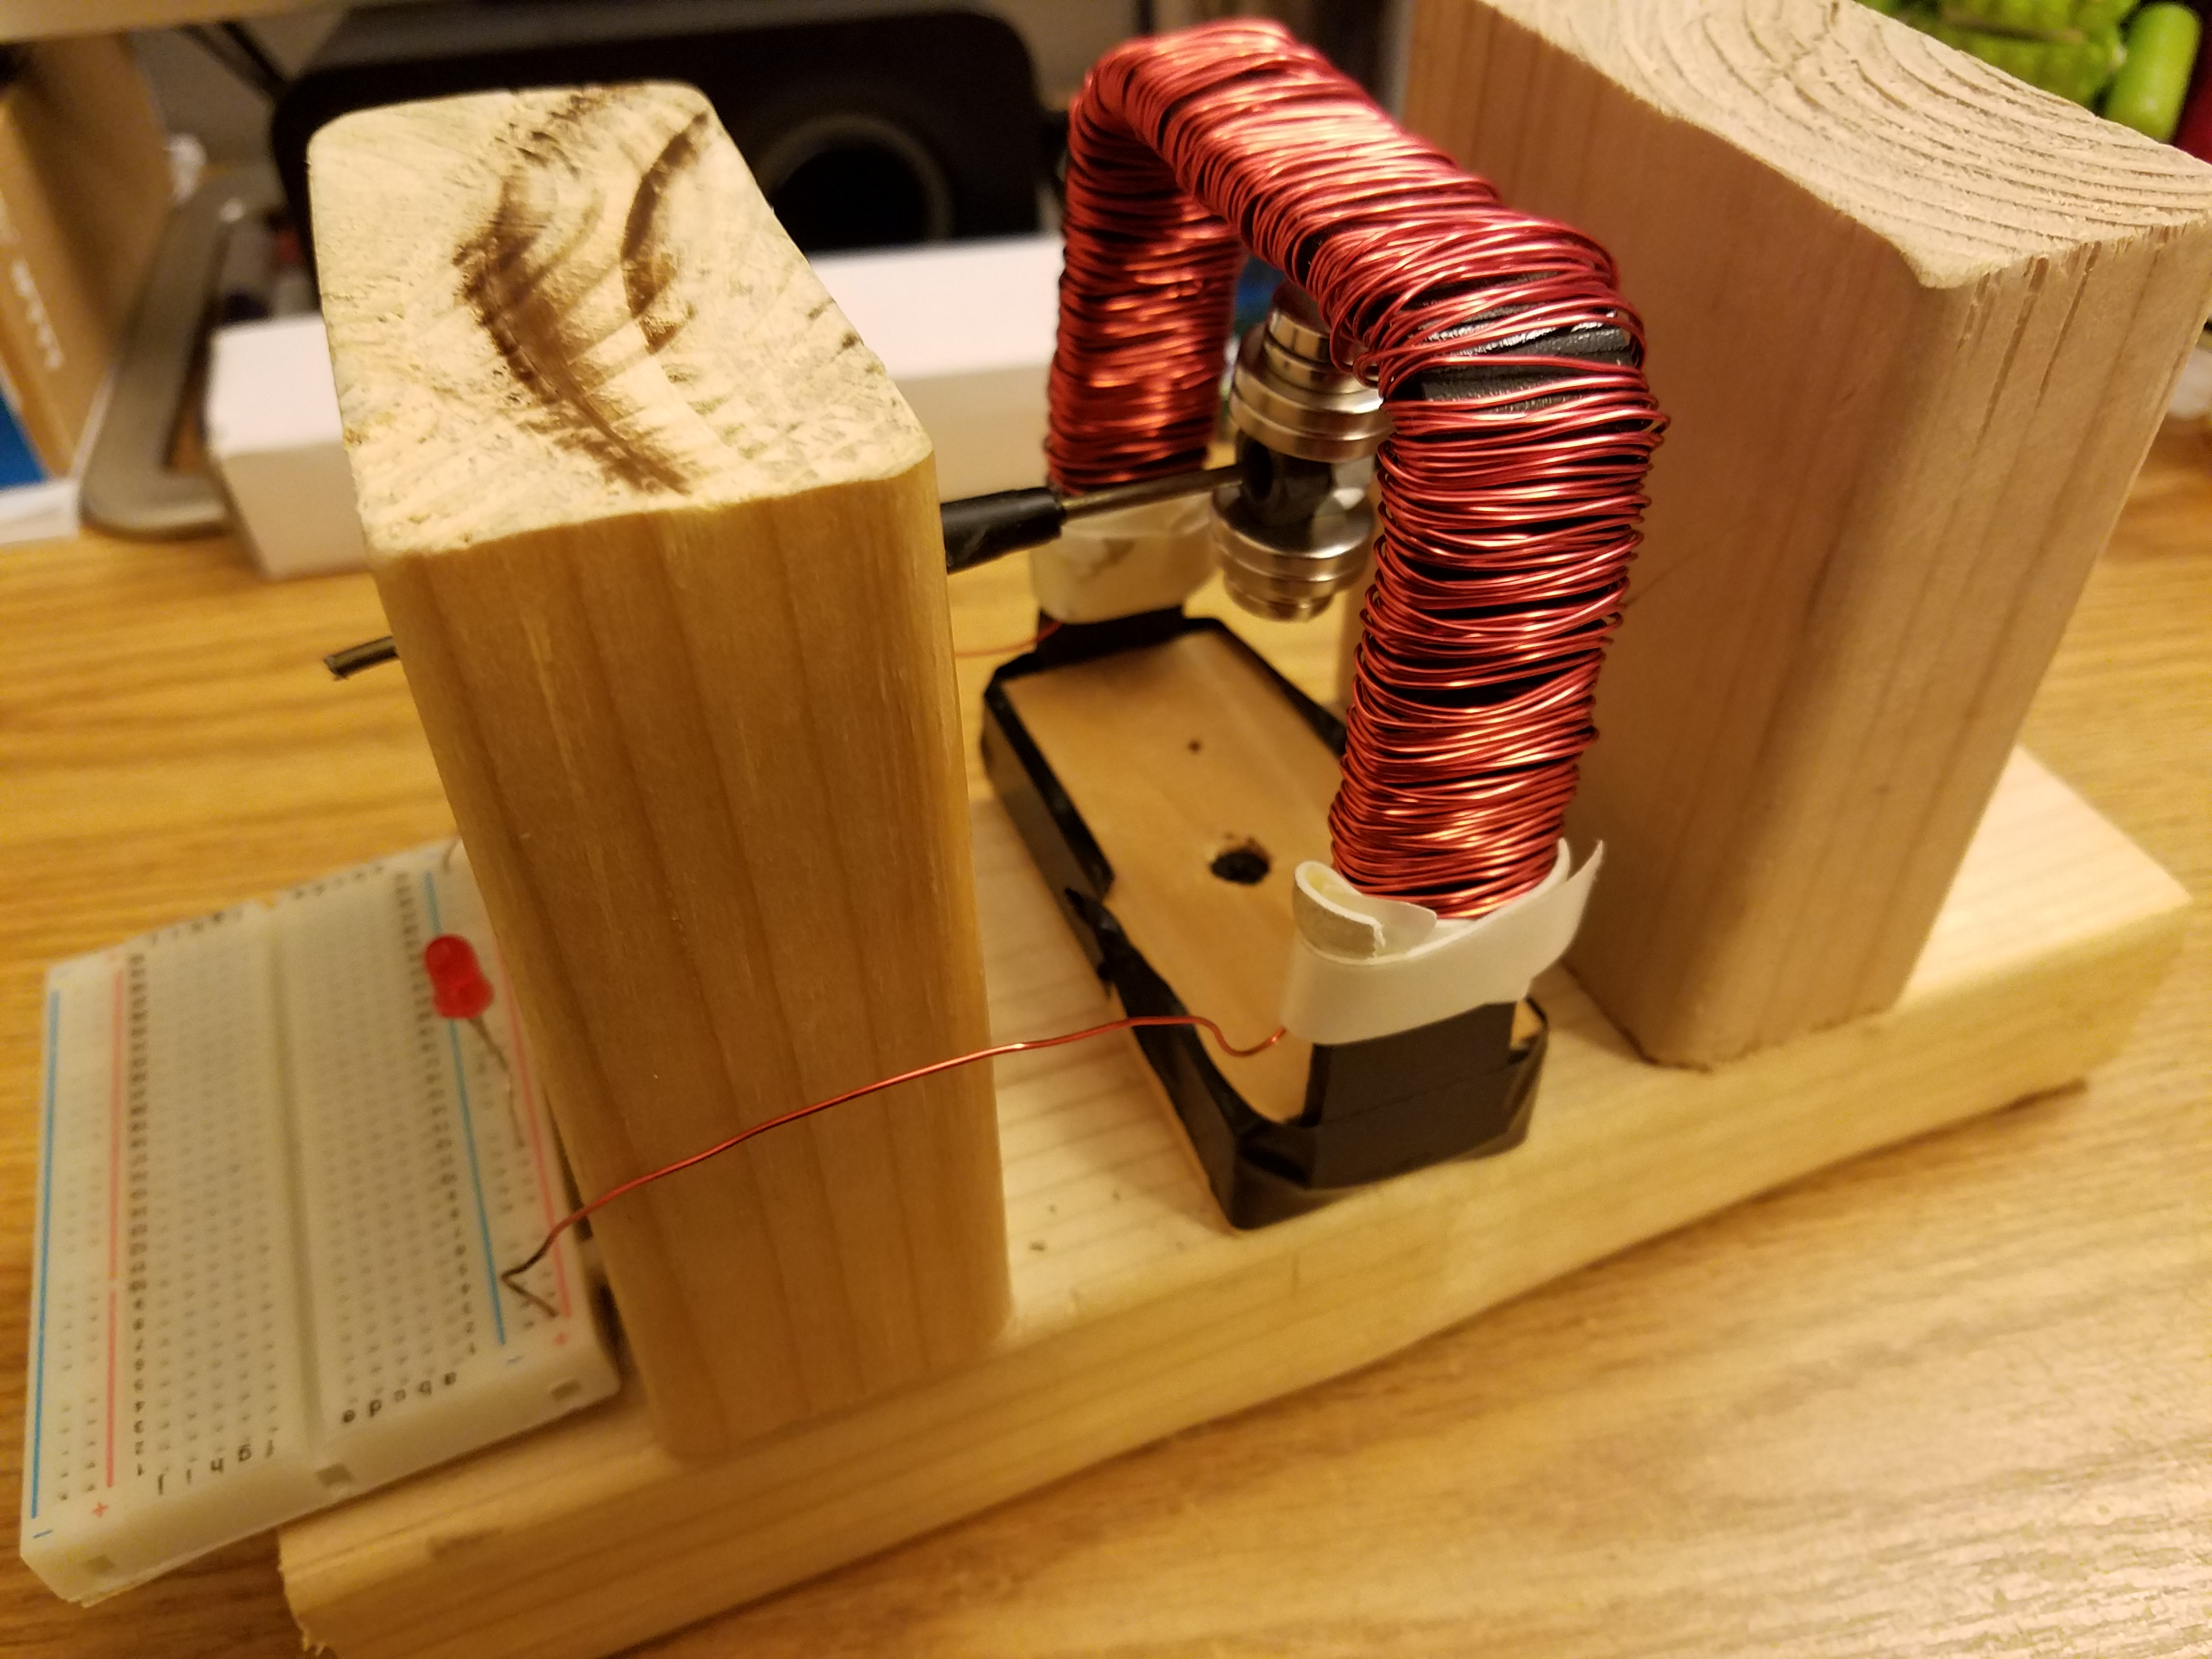
\includegraphics[width=0.6\textwidth]{figures/models/5.jpg}
            \label{fig:model5}
        \end{center} \caption{Final Model Demonstrated during Presentation}
    \end{figure}

    \noindent
    After the failed attempts to build a reciprocal project, a final model was designed with the idea of spinning the coils through a stationary magnetic field. The input voltage was upgraded to 22 V, bigger and stronger N52 neodymium magnets were obtained, and a sturdier frame was constructed. When being tested, the coil successfully spun in the magnetic field when the current was allowed to flow through. A power drill was also used to spin the armature to generate almost 120 mV.\\

    \begin{figure}[ht]
        \begin{center}
            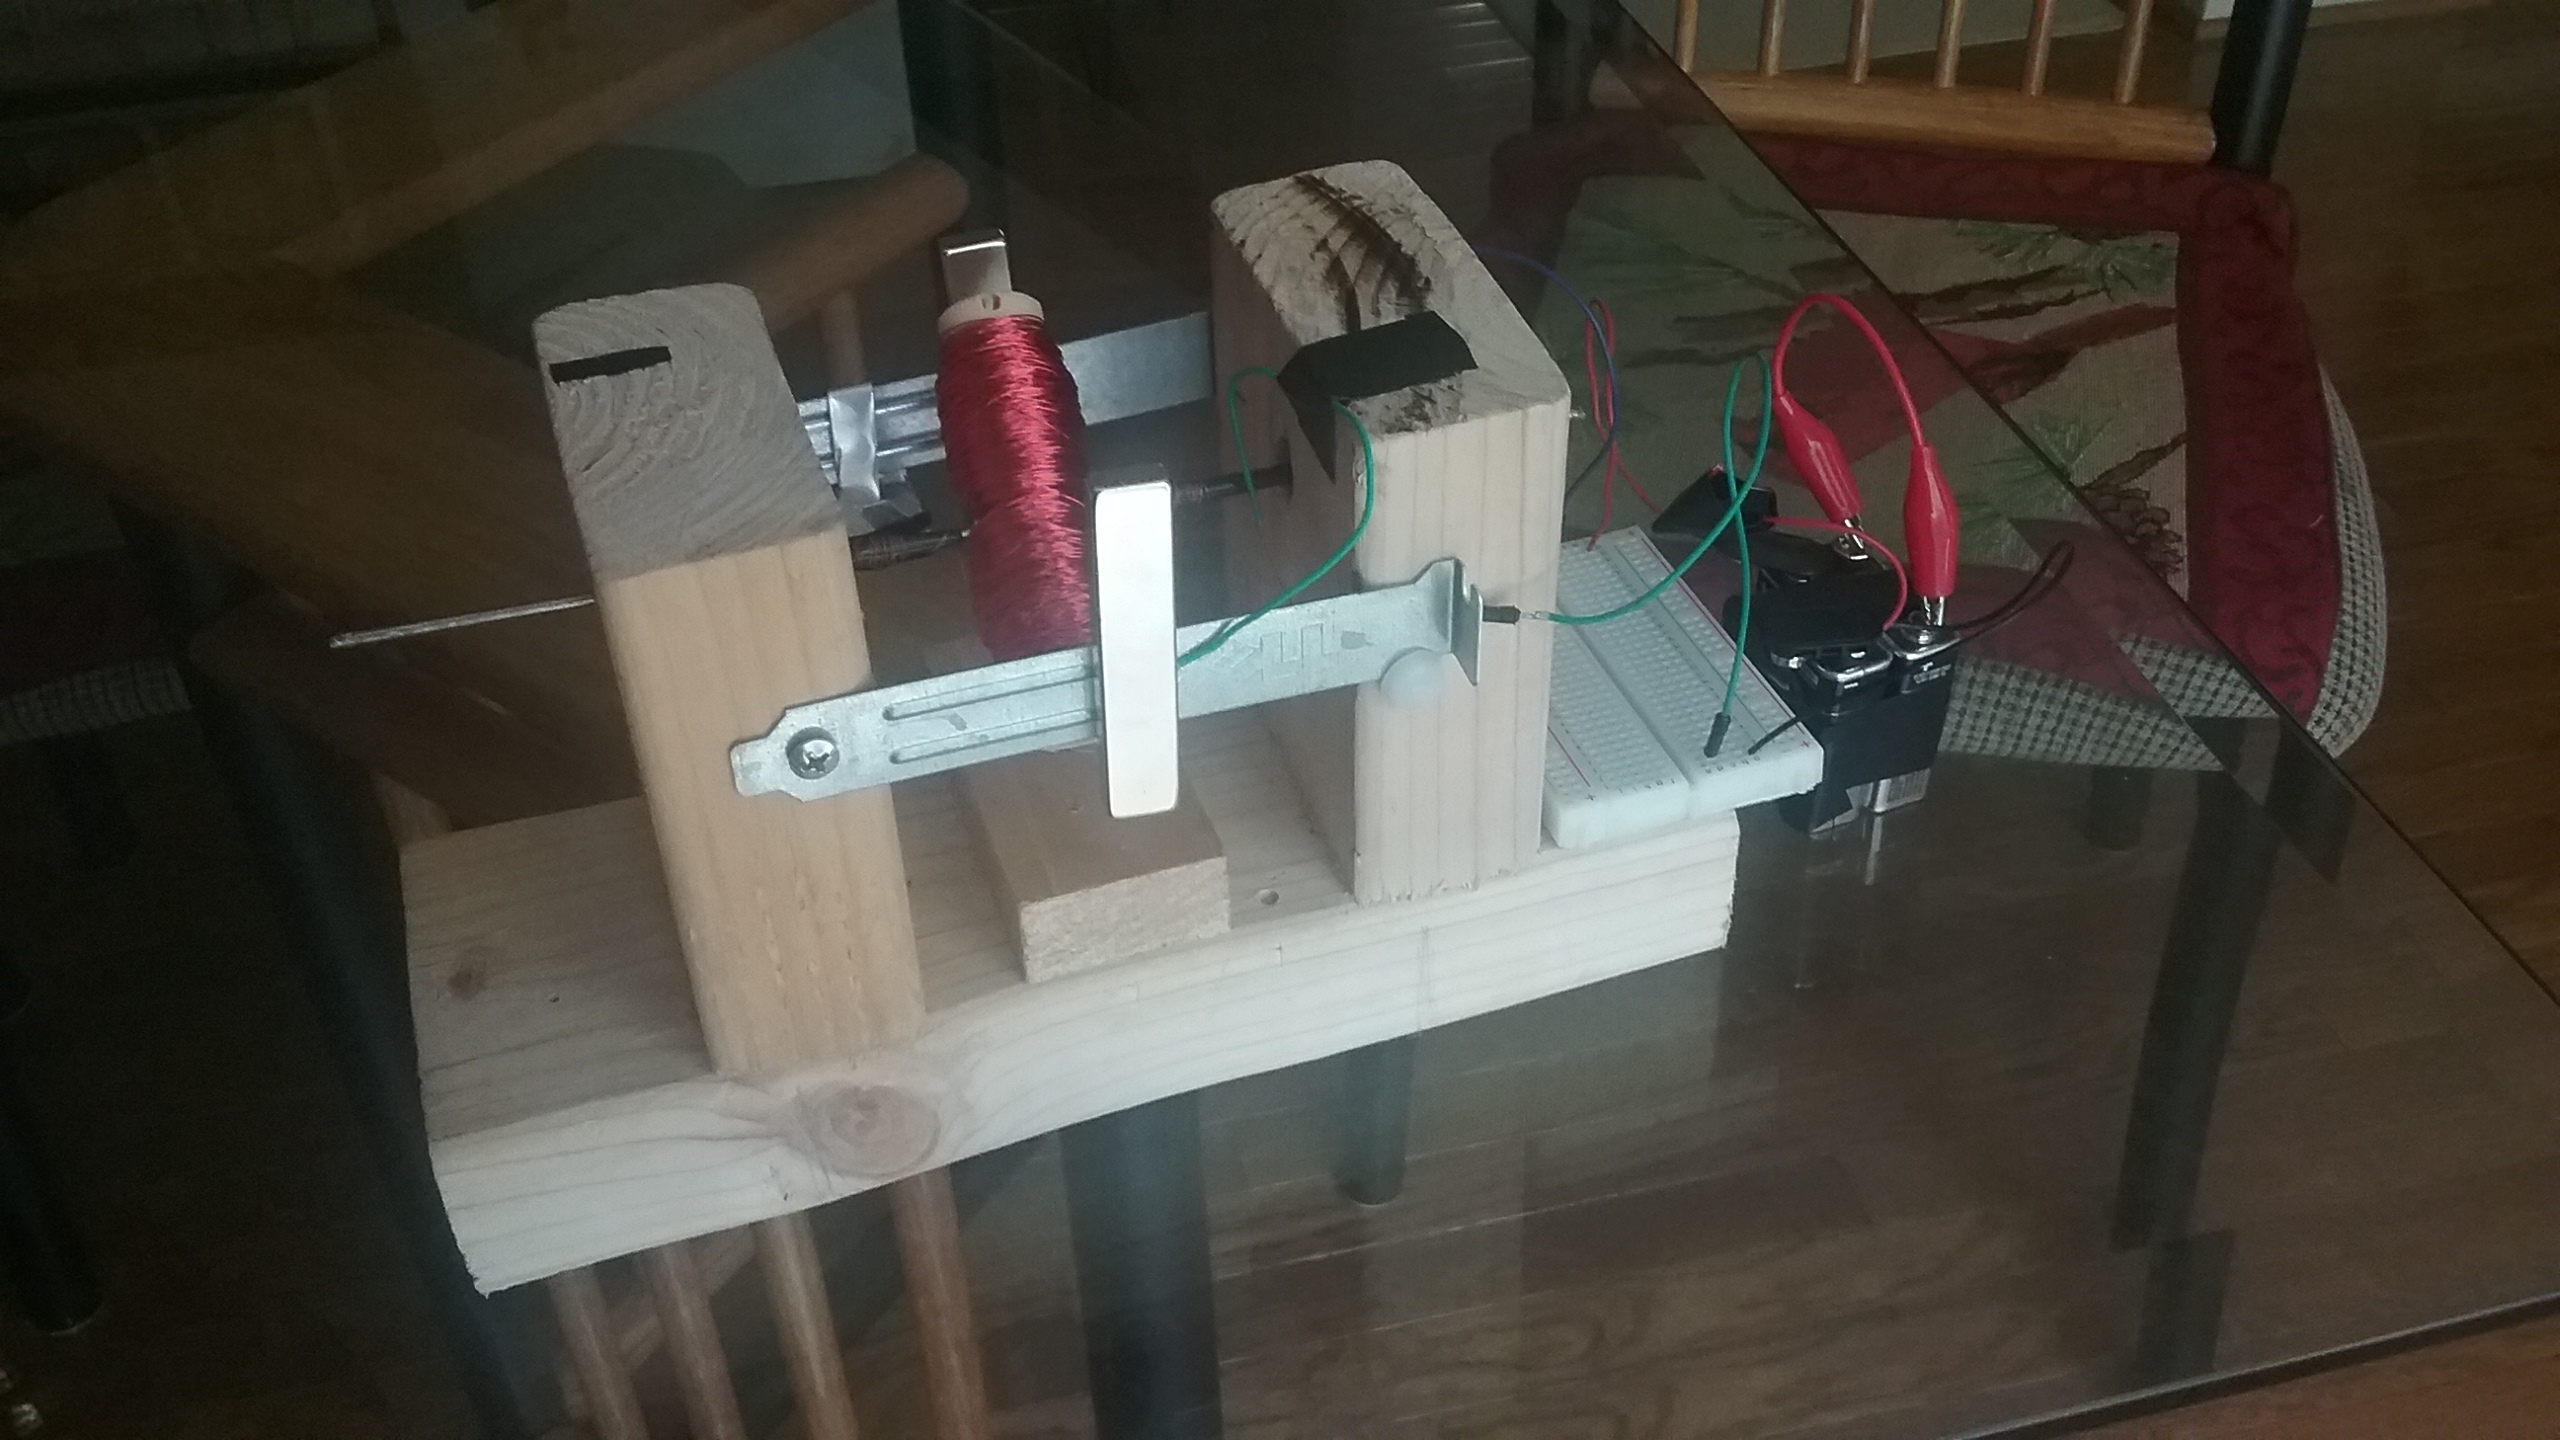
\includegraphics[width=0.6\textwidth]{figures/models/6.jpg}
            \label{fig:model6}
        \end{center} \caption{Last Model as a Second Attempt}
    \end{figure}

    \noindent
    However, the model was tested with multiple members of the team manually holding the leads to act as brushes on the commutators. Constructing the brushes to build a stable, standalone model proved to be the most difficult task. Getting a conductive material to make physical contact with a simple commutator half insulated with duct tape did not appear feasible with the limited materials available. The errors caused by imperfect measurements of the angles and lengths of the brushes and their support mechanisms caused the model to fail to be demonstrated.
